\pagenumbering{arabic}%DO NOT REMOVE THIS
\chapter{Introduction and Background}\label{ch:intro}
Some species of bacteria have experienced reductive evolution over the course of millions of years, and this reduction in their genome has lead to a loss of genes, regulatory abilities, etc. The reasons for this are an area of active research %TODO insert citation for current research
, though it is often difficult or impossible to reproduce the natural environmental conditions in a lab in order to study this. As an alternative, \textit{in silico evolution} is one option that can be used to study the conditions under which an organisms genome may reduce. In this method, organisms and their evolution over thousands or millions of generations are simulated in software. In this manner, one can control and evaluate every aspect of their evolution over time, and a full record of their lineage may be maintained and studied, potentially leading to a greater understanding of the factors that lead to specific effects on the genome. The in silico tool \textit{Aevol} is one such platform which realistically models bacterial genomes and evolution, allowing one to draw conclusions about their real-world counterparts. In the following thesis, we present the results of our experiments in artificial evolution which aim to identify and evaluate several factors which potentially lead to changes in genome structure and potentially a reduced genome in simulated bacteria using the aevol platform. 

\section{Problem Statement}
Among the difficulties of studying reductive evolution with in vivo evolutionary experiments, one of the most difficult obstacles to overcome is the lack of a full ancestral record. This lack of a full phylogeny can make it difficult or impossible to tell exactly when and how a specific trait evolved, as illustrated in Figure \ref{fig:phylogeny03} below. 
\begin{figure}[h]\label{fig:phylogeny03}
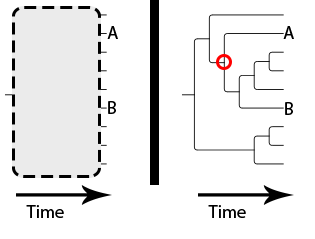
\includegraphics[scale=0.75]{phylogeny03}
\centering
\caption{An illustration of unknown phylogeny. The information under the shaded box is not known, such as the point of divergence (red circle).}
\end{figure}
In this example, if we are comparing two related organisms, A and B, and we are trying to determine when a specific trait was gained or lost by one of the organisms (e.g. to determine its relative importance due to conservation over many generations), without the phylogenetic information (under the shaded box) we may not be able to identify the point in their evolutionary history at which the two organisms diverged, making estimates difficult or impossible.

Another major downside to \textit{in vivo} evolutionary experiments is that they are slow. For example, the relatively well-known E. coli Long-Term Evolution Experiment (LTEE) by Profesor Lenski at Michigan State University has been ongoing since February of 1988 and only passed generation 65,000 in 2016, 28 years later. 

As an alternative to in vivo, in silico evolutionary experiments are well-suited to the task of studying reductive evolution. Generations of organisms may be evolved within a very short time period, and a full "fossil record" of each lineage may be kept on disk for further analysis. 

The in silico tool Aevol has a realistic artificial chemistry model which was developed specifically to study genome structure. It contains tools to analyze the robustness, fitness, and evolvability of digital organisms over time. 

\subsection{Report outline}
This chapter serves as the introduction to the thesis and the research problem we are facing. In Chapter~\ref{ch:background}, we provide some necessary background information on in silico evolution in general and aevol in particular. Chapter~\ref{ch:approach} describes our experimental setup. Chapter~\ref{ch:results_discussion}
provides the results and analysis of the experiments, and Chapter~\ref{ch:conclusion} gives our conclusions. 

In this section we provide some general background information about in silico evolution and aevol, the artificial evolution platform used in our experiments. 

